%! Author = Kevin Häusler
%! Date = 08/11/2024

% Preamble
\documentclass[11pt,a4paper]{article}
% Packages
\usepackage[utf8]{inputenc}       % accents
\usepackage[T1]{fontenc}          % PS fonts
\usepackage{newtxtext,newtxmath}  % do not use CM fonts
\usepackage{amsmath}              % multi-line and other mathematical statements
\usepackage{setspace}             % setting the spacing between lines
\usepackage{graphicx}             % go far beyond what the graphics package
\usepackage[normalem]{ulem}       % various types of underlining
\usepackage{caption}              % rotating captions, sideways captions, etc.
\usepackage{float}                % tables and figures in the multi-column environment
\usepackage{subcaption}           % for subfigures and the like
\usepackage{longtable}            % tables that continue to the next page
\usepackage{multirow}             % tabular cells spanning multiple rows
\usepackage[table]{xcolor}        % driver-independent color extensions
\usepackage{lipsum}               % loren dummy text
\setlength{\marginparwidth}{2cm}  % todonotes' requirements
\usepackage{todonotes}            % todo's
\usepackage{csquotes}             % context sensitive quotation facilities
\usepackage[backend=biber,authordate]{biblatex-chicago}  % Chicago Manual of Style

%% document dimensions
\usepackage[a4paper, left=25mm,right=25mm,top=25mm,bottom=25mm,headheight=6mm,footskip=12mm]{geometry}
\setlength{\parindent}{0em}
\setlength{\parskip}{1ex}

%% headers & footers
\usepackage{lastpage}
\usepackage{fancyhdr}
\fancyhf{}                            % clear off all default fancyhdr headers and footers
\rhead{\small{\emph{\projtitle, \projauthor}}}
\rfoot{\small{\thepage\ / \pageref{LastPage}}}
\pagestyle{fancy}                     % apply the fancy header style
\renewcommand{\headrulewidth}{0.4pt}
\renewcommand{\footrulewidth}{0.4pt}

%% colors
\usepackage{color}
\definecolor{engineering}{rgb}{0.549, 0.176, 0.098}
\definecolor{cloudwhite}{cmyk}{0,0,0,0.025}
%% quotes
\usepackage{dirtytalk}
%% source-code listings
\usepackage{listings}
\lstset{ %
 language=C,                        % choose the language of the code
 basicstyle=\footnotesize\ttfamily,
 keywordstyle=\bfseries,
 numbers=left,                      % where to put the line-numbers
 numberstyle=\scriptsize\texttt,    % the size of the fonts that are used for the line-numbers
 stepnumber=1,                      % the step between two line-numbers. If it's 1 each line will be numbered
 numbersep=8pt,                     % how far the line-numbers are from the code
 frame=tb,
 float=htb,
 aboveskip=8mm,
 belowskip=4mm,
 backgroundcolor=\color{cloudwhite},
 showspaces=false,                  % show spaces adding particular underscores
 showstringspaces=false,            % underline spaces within strings
 showtabs=false,                    % show tabs within strings adding particular underscores
 tabsize=2,                         % sets default tabsize to 2 spaces
 captionpos=t,                      % sets the caption-position to top
 belowcaptionskip=12pt,             % space between caption and listing
 breaklines=true,                   % sets automatic line breaking
 breakatwhitespace=false,           % sets if automatic breaks should only happen at whitespace
 escapeinside={\%*}{*)},            % if you want to add a comment within your code
 morekeywords={*,var,template,new}  % if you want to add more keywords to the set
}

%% hyperreferences (HREF, URL)
\usepackage{hyperref}
\hypersetup{
    plainpages=false,
    pdfpagelayout=SinglePage,
    bookmarksopen=false,
    bookmarksnumbered=true,
    breaklinks=true,
    linktocpage,
    colorlinks=true,
    linkcolor=engineering,
    urlcolor=engineering,
    filecolor=engineering,
    citecolor=engineering,
    allcolors=engineering
}

%% path to the figures directory
\graphicspath{{figures/}}

%% bibliography file, must be in preamble
\addbibresource{bibliography.bib}

%% macros, to be updated as needed
\newcommand{\school}{HSLU: Lucerne University of Appplied Sciences and Arts}
\newcommand{\degree}{BSC Artificial Intelligence and Machine Learning}
\newcommand{\projtitle}{DVIZ Main Project}
\newcommand{\projauthor}{Kevin Häusler}
\newcommand{\tutor}{Prof.\ Elena Nazarenko, PhD}

%% my other macros, if needed
\newcommand{\windspt}{\textsf{WindsPT\/}}
\newcommand{\windscannerpt}{\emph{Windscanner.PT\/}}
\newcommand{\class}[1]{{\normalfont\sffamily #1\/}}
\newcommand{\svg}{\class{SVG}}

%% my environments for infos
\newenvironment{info}[1]{\vspace*{6mm}\color{blue}[ \textbf{INFO:} \begin{em} #1}
                        {\vspace*{3mm}\end{em} ]}
\newenvironment{infoopt}[1]{\vspace*{6mm}\color{blue}[ \textbf{INFO (elemento opcional):} \begin{em} #1}
                        {\vspace*{3mm}\end{em} ]}

%%------------------------------- document-------------------------------------

\begin{document}

%% preamble page numbers with arabic numerals
\pagenumbering{arabic}\setcounter{page}{1}

%%------------------------------- cover page ----------------------------------

\begin{titlepage}
\center

\vspace{-15mm}
{\large \textbf{\textsc{\school}}}\\

\vfill

{\Large \textbf{\projtitle}}\\[8mm]

{\Large \textbf{\projauthor}}\\

\vfill

%\includegraphics[width=52mm]{uporto-feup.pdf}

\vfill

{\large \degree}\\[8mm]
{\large \textbf{Tutor}: \tutor}\\[8mm]

%\renewcommand{\today}{15 de dezembro de 2023}
\today

\end{titlepage}

%%------------------------------- table of contents ---------------------------

%% redefine tableofcontents text, ONLY for PT
\renewcommand{\contentsname}{Table of Contents}

\tableofcontents
\newpage

%%------------------------------- table of work ---------------------------
\section{Work Table}

Due to me (Kevin Häusler) being the sole member of this project I have omitted the "done by" column.

\begin{table}[H]
\centering
\begin{tabular}{|l|l|l|}
\hline
\textbf{Date} & \textbf{Hours} & \textbf{Task description} \\ \hline
22.10.2024 & 1 & Downloading 9k Dataset from Shodan \\ \hline
07.11.2024 & 1 & Setup the project, convert the json data to xlsx, setup latex environment \\ \hline
07.11.2024 & 1 & Configure the initial streamlit setup \\ \hline
08.11.2024 & 1 & Start writing the report + setup Github \\ \hline
15.11.2024 & 2 & Research about Shodan\\ \hline
23.11.2024 & 1 & Writing more functions in the code\\ \hline
08.12.2024 & 1 & Downloading new 32k Dataset from Shodan \\ \hline
08.12.2024 & 2 & Analysis of the new 32k Dataset \\ \hline
09.12.2024 & 4 & Code Refactor and Data Analysis \\ \hline
10.12.2024 & 1 & Update Report, start working on Hosting of Project \\ \hline



\end{tabular}
\end{table}

\newpage

%%------------------------------- About the  Project ---------------------------
\begin{about}
\section{About the Project}
\subsection{What is the project?}
The project is something akin to a cyber security analytic about the devices listed on shodan.io based on their location
being Rotkreuz. It is supposed to show insights about what is accessible and possibly insecure.

There are also dynamic parts where you can filter the data.
\subsection{Data}
The data is generated from shodan.io. I do have a lifetime membership that grants me enough credits to request and
download 10'000 entries. I did filter the data to be only from Rotkreuz which resulted in a little bit over 9000
datapoints that I am using for this project.

Why I am not using the entire 32'000 dataset is explained in my report where I go indepth about how I got the data.

\subsection{Tools}
Here is a list of the tools I am using:

PyCharm \\
Python 3.11 \\
UV \\
Streamlit \\
Shodan CLI \\
Docker \\
Github \\
LaTeX \\

I have setup the project in pycharm with UV so it is easier to distribute, there is also a docker file in case you have
docker installed to easily run this project without having to create your own environment.

For the main library I have decided to use Streamlit, I have tried it out in the past but never for a real project so I
wanted to get more indepth experience with it. It has a great documentation and it lets me easily create dataframes and
charts for this project.

The whole report is also written in the PyCharm IDE with LaTeX and uploaded to the Github repository. It is written in the
report.tex file and compiled to report.pdf.

This setup is also useful in case I need to work from different machines.

\subsection{Shodan}

Shodan.io or more commonly referred as just Shodan is a search engine tool used to provide a more comprehensive view of
the internet, more specifically it crawls, scans and collects information from a wide range of devices that are public to
the internet.

This includes servers, IOT devices, webcams, routers even industrial control systems.

This data can be browsed and used to "help" assess cybersecurity risks. It does not guarantee that your systems are secure or insecure,
so do not mistake it as being a complete cybersecurity assessment.

I was lucky enough to get a "lifetime" membership for 5 USD, this gives me access to multiple tools and 100 query credits.

1 Query credit corresponds to 100 results which is why my initial dataset to try out the feasibility of this project only
contains 9000 datapoints. For this project I decided to sign up for a freelancer membership so I get 10´000 query credits
which I can use to get the entire dataset of Rotkreuz and maybe implement an interactive tool as well with the Shodan API.

\end{about}
\newpage

%%------------------------------- motivation ---------------------------
\begin{motivation}
\section{Motivation}
The main motivation of this project was to use shodan.io and streamlit to create something interesting. I have rarely used
my shodan membership which felt bad even though I only paid 5 USD for a lifetime membership.

Streamlit has been something I have been trying out for a personal project but I never really got into it as much as I
would have liked due to other commitments.

\subsection{Cyber Security}
Another relevant motivation would be cyber security. This semester I am taking the Introduction to Cyber Security class
which has been surprisingly fun and interesting. While this project does not equal to a real cyber security assessment I
do want to try my best to create something that is informative and useful in that regard.

\end{motivation}
\newpage

%%------------------------------- research ---------------------------
\begin{research}
\section{Research}


\subsection{A Study on Internet of Things Devices Vulnerabilities using Shodan}
There is a short research paper about the vulnerabilities of IOT devices where the author used shodan as a search engine
to get the required data for his research.

\subsection{Guides on how to use Shodan}
There are many interesting and informative articles on medium.com and cyber security blogs about how to leverage Shodan
for cyber security or more "nefarious" purposes like gaining access to unsecured webcams and NAS.

\subsection{Using Shodan to hunt down Ransomware Groups}
One of my favorite cybersecurity researcher and youtuber John Hammond is affiliated with the cybersecurity firm Huntress,
which is how I came upon a blog post about using Shodan to hunt down Ransomware groups.

While it is not entirely relevant to my project it has been a very interesting read and I can recommend it for people that
are interested in this.

https://www.huntress.com/blog/using-shodan-images-to-hunt-down-ransomware-groups


\end{research}
\newpage

%%------------------------------- data ---------------------------
\begin{data}
\section{Data}
\subsection{Getting the Data}

As mentioned I will be using Shodan to get the data about all the devices that are scanned in Rotkreuz.

This is done with their search engine tool on https://www.shodan.io/search?query=country%3A%22CH%22+city%3A%22rotkreuz%22

\begin{figure}[!htb]
    \centering
    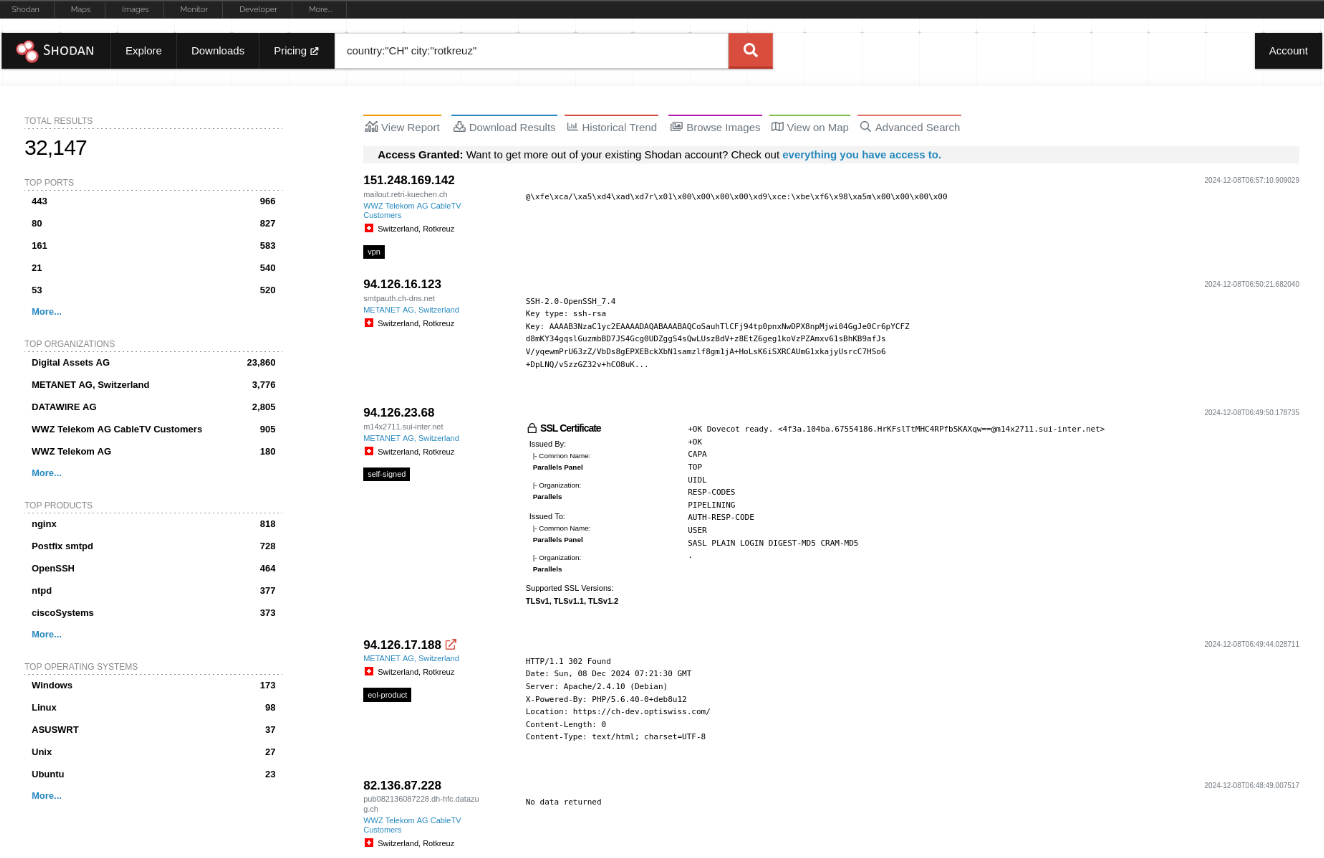
\includegraphics[width=\textwidth,height=\textheight,keepaspectratio]{/home/kevin/images/shodan-search-results}
    \caption{Shodan Search Results for Rotkreuz CH}
    \label{fig:shodan-search-results}
\end{figure}

Here we can see 32'147 results which I downloaded.

\begin{figure}[!htb]
    \centering
    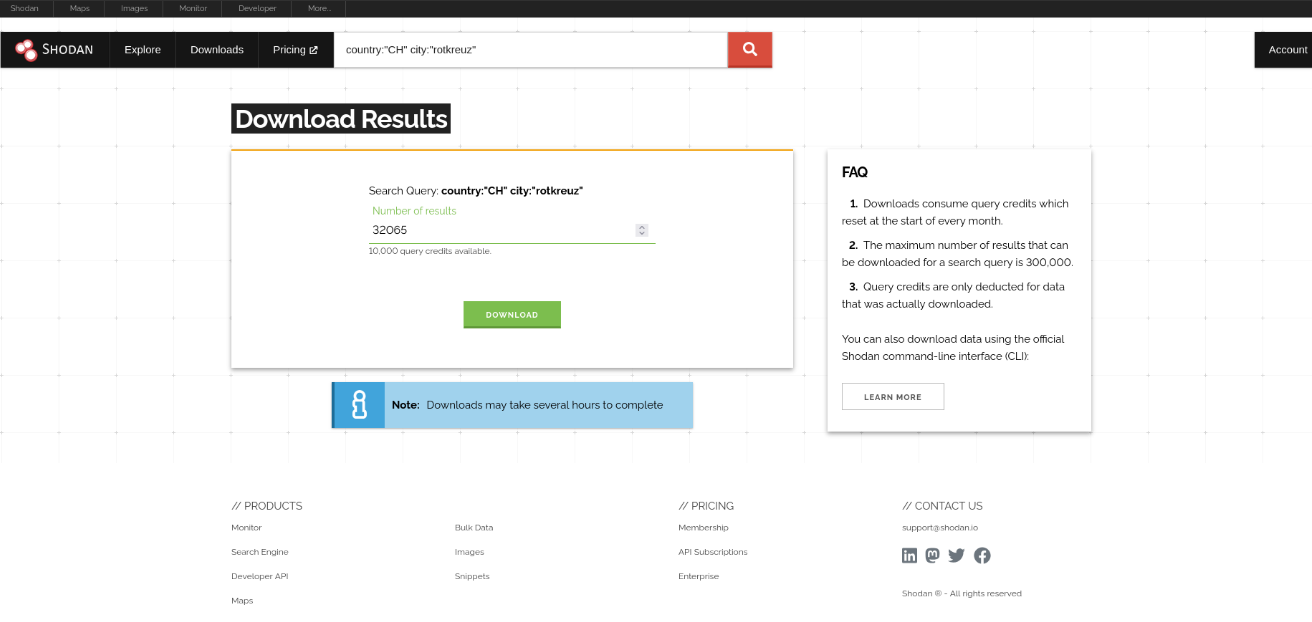
\includegraphics[width=\textwidth,height=\textheight,keepaspectratio]{/home/kevin/images/shodan-download-page}
    \caption{Downlaoding the search results}
    \label{fig:shodan-download-page}
\end{figure}


\subsection{Preparing the Data}

The download returns a *.json.gz archive which I have renamed to shodan\textbf{\textunderscore}data\textbf{\textunderscore}unprepped.json.gz for this project.

\begin{figure}[!htb]
    \centering
    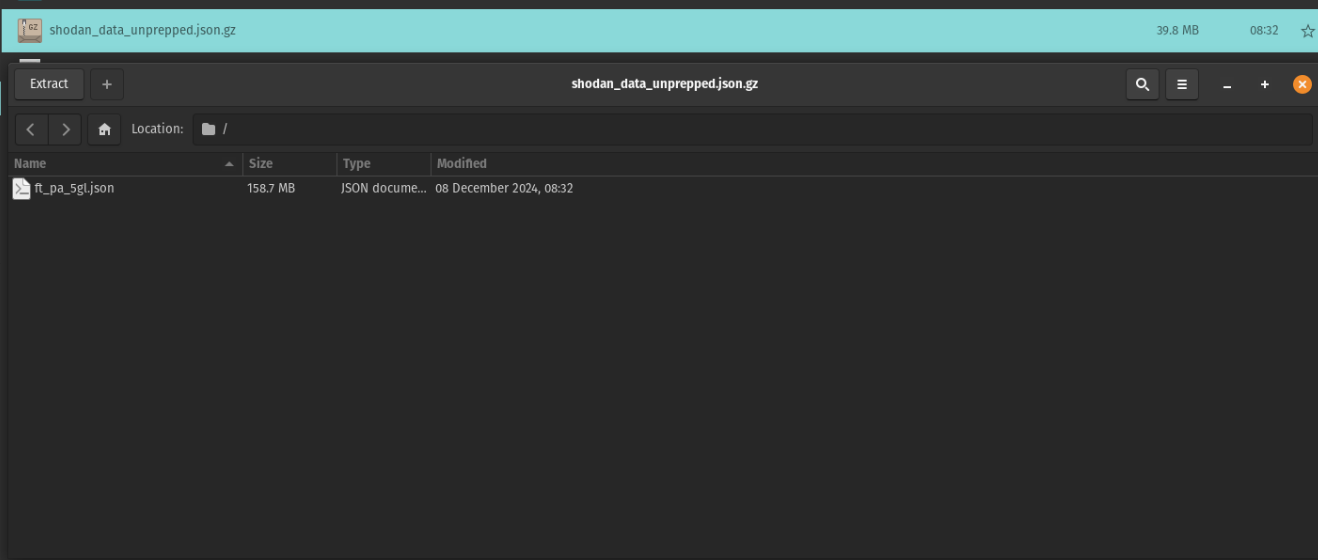
\includegraphics[width=\textwidth,height=\textheight,keepaspectratio]{/home/kevin/images/downloaded-archive}
    \caption{The Downloaded Archive}
    \label{fig:downloaded-archive}https://www.shodan.io/search?query=country%3A%22CH%22+city%3A%22rotkreuz%22+org%3A%22Digital+Assets+AG%22&page=3
\end{figure}

We can convert this with the following command: "convert shodan\textbf{\textunderscore}data\textbf{\textunderscore}unprepped.json.gz xlsx to an xlsx file which we rename to shodan\textbf{\textunderscore}data\textbf{\textunderscore}32k.xlsx.


\newpage
\subsubsection{Unexpected Issue}
But what is this? We suddenly have a lot  (27'768) of N/A entries in our dataset.

\begin{figure}[h!]
    \centering
    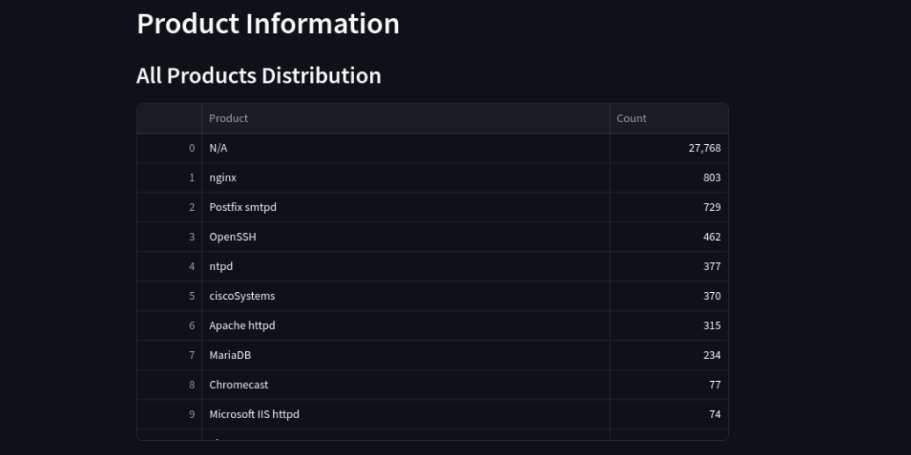
\includegraphics[keepaspectratio,scale=0.3]{/home/kevin/images/32k-dataset-na-entries}
    \caption{27´000 N/A with the 32k Dataset}
    \label{fig:32k-dataset-na-entries}
\end{figure}

When I compare this with the 9k Dataset that I downloaded on 22.10.2024 we only have 4'643 N/A entries.

\begin{figure}[h!]
    \centering
    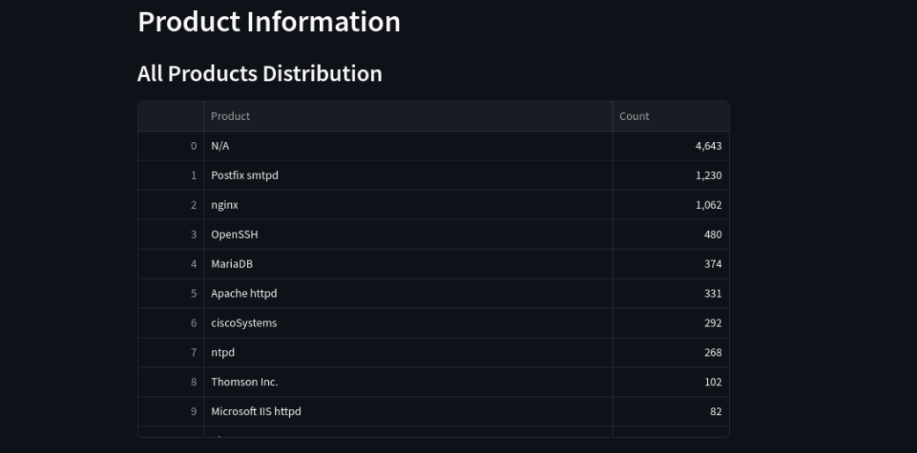
\includegraphics[keepaspectratio,scale=0.3]{/home/kevin/images/9k-dataset-na-entries}
    \caption{Only 4'643 N/A with the 9k Dataset}
    \label{fig:9k-dataset-na-entries}
\end{figure}

\newpage

An indepth look at the Shodan search engine shows an organisation called Digital Assets AG with 23'860 datapoints, and
while they have a lot of open ports they do not return any data.

\begin{figure}[h!]
    \centering
    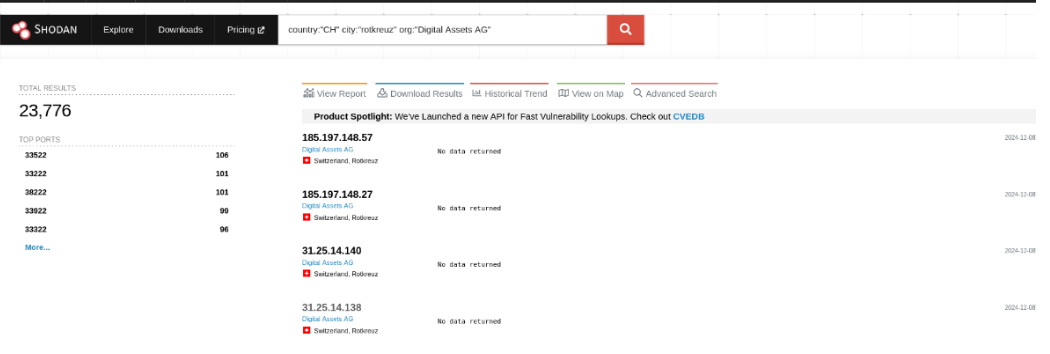
\includegraphics[keepaspectratio,scale=0.3]{/home/kevin/images/digital-assets-ag-rotkreuz-ch-search}
    \caption{Digital Assets AG Rotkreuz CH Search}
    \label{fig:digital-assets-ag-rotkreuz-ch-search}
\end{figure}

An overview of one of these IP can be looked at here https://www.shodan.io/host/185.197.148.27


When we look at the company itself we can see that they have 77'280 servers in Germany

\begin{figure}[h!]
    \centering
    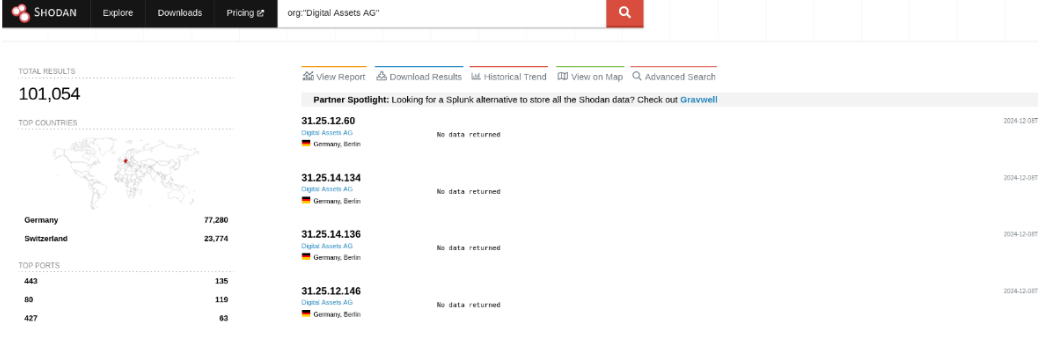
\includegraphics[keepaspectratio,scale=0.3]{/home/kevin/images/shodan-digital-assets-ag}
    \caption{Shodan Digital Assets AG}
    \label{fig:shodan-digital-assets-ag}
\end{figure}

The ASN lookup confirms that it is part of the Google Cloud Platform. While I do not have any confirmation it is highly likely that
they are renting or colocating servers (in this case VPS) in the new CKW Datacenter in Rotkreuz.

To be safe I will use the 9k dataset from 22.10.2024 for this project.

\subsection{Analyzing the Data}
Now that we have our data we an start analyzing it. First I want to check some general information like:
- What are the most common ports?
- What are the most common used Software
- Are there any weird/interesting findings that stand out?

\newpage
\subsubsection{Port Distribution}
A closer look at the Port distribution shows that the main use is web (port 443 and 80) and email services (port 25). There are
some concerning ports like DNS (53) that are not recommended to be accessible publicly.

This can be exploited by using the exposed DNS servers to DDoS other systems by sending tons of fake DNS responses in a DNS amplification attack.

Thankfully most of the exposed DNS ports are from web hosting companies and datacenters that should know the risks and how to prevent them.
There are still 19 open DNS Ports from WWZ ISPs that could be residential that are worrisome.

\begin{figure}[!h]
    \centering
    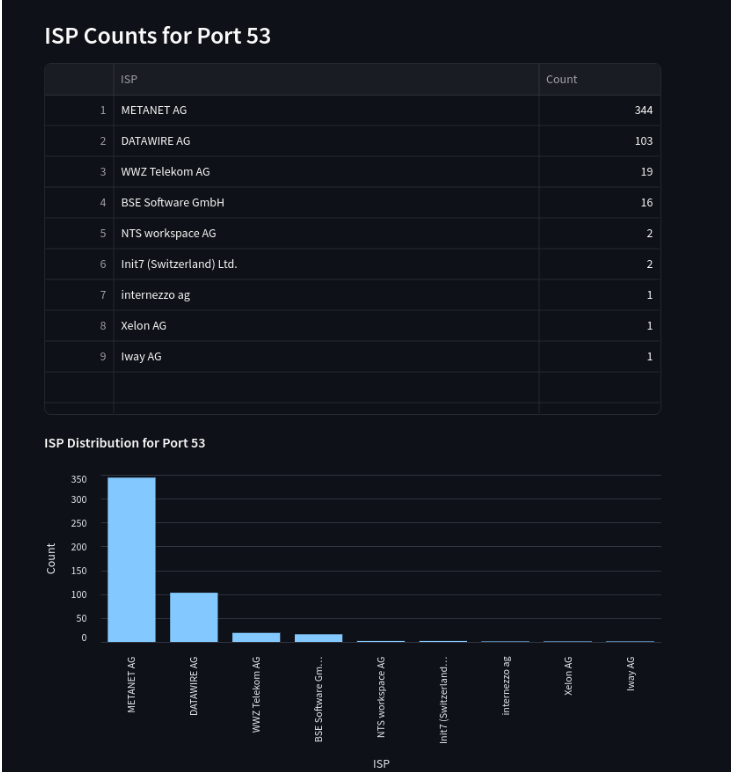
\includegraphics[keepaspectratio,scale=0.3]{/home/kevin/images/port-53-distribution-by-isp}
    \caption{Port 53 Distribution by ISP}
    \label{fig:port-53-distribution-by-isp}
\end{figure}


\end{data}
\newpage
\end{document}